% Source: graduate-coursework/Sp26/CSCE763/Course_Assignments/Project/project_proposal.tex
% Description: Faster R-CNN two-stage architecture with radar-specific anchor optimization and scale normalization for range-dependent target size variation.

\documentclass[border=4pt]{standalone}
\usepackage{amsmath}
\usepackage{amssymb}
\usepackage{graphicx}
\usepackage{tikz}
\usepackage{xcolor}
\usetikzlibrary{positioning, arrows.meta, calc, fit, backgrounds, decorations.pathreplacing}

\definecolor{USC_Garnet}{HTML}{73000A}
\definecolor{USC_Black10}{HTML}{ECECEC}
\definecolor{USC_Black70}{HTML}{5C5C5C}
\definecolor{USC_Congaree}{HTML}{1F414D}

\begin{document}
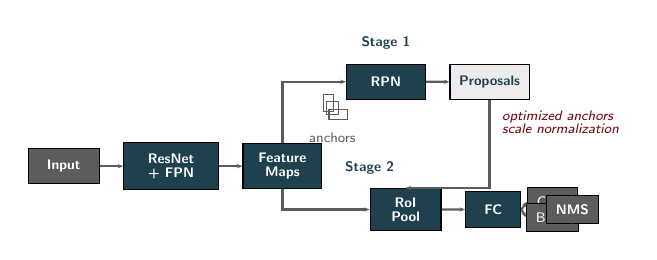
\begin{tikzpicture}[
  scale=0.72, every node/.style={font=\sffamily\tiny},
  block/.style={draw, fill=USC_Congaree, text=white, minimum height=0.45cm,
    minimum width=0.9cm, font=\sffamily\tiny\bfseries, align=center},
  nblock/.style={draw, fill=USC_Black70, text=white, minimum height=0.45cm,
    minimum width=0.9cm, font=\sffamily\tiny\bfseries, align=center},
  bgblock/.style={draw, fill=USC_Black10, minimum height=0.45cm,
    minimum width=0.9cm, font=\sffamily\tiny\bfseries, align=center,
    text=USC_Congaree},
  arr/.style={-{Stealth[length=2pt]}, thick, USC_Black70}
]
  % Input
  \node[nblock, minimum width=0.9cm] (inp) {Input};

  % Backbone
  \node[block, right=0.3cm of inp, minimum width=1.2cm, minimum height=0.6cm] (back)
    {ResNet\\[-1pt]+ FPN};

  % Feature maps
  \node[block, right=0.3cm of back, minimum width=1.0cm, minimum height=0.55cm] (feat)
    {Feature\\[-1pt]Maps};

  % Stage 1: RPN branch (above)
  \node[block, above right=0.55cm and 0.3cm of feat, minimum width=1.0cm] (rpn)
    {RPN};

  % Anchor boxes illustration near RPN
  \draw[USC_Black70, thin] ([xshift=-0.35cm, yshift=-0.25cm]rpn.south west)
    rectangle ++(0.22cm,0.22cm);
  \draw[USC_Black70, thin] ([xshift=-0.3cm, yshift=-0.35cm]rpn.south west)
    rectangle ++(0.32cm,0.18cm);
  \draw[USC_Black70, thin] ([xshift=-0.4cm, yshift=-0.2cm]rpn.south west)
    rectangle ++(0.18cm,0.3cm);
  \node[USC_Black70, font=\sffamily\tiny, anchor=north]
    at ([xshift=-0.24cm, yshift=-0.4cm]rpn.south west) {anchors};

  % Proposals
  \node[bgblock, right=0.3cm of rpn, minimum width=0.9cm] (prop) {Proposals};

  % Stage 2: RoI Pooling (below, connecting from feat and proposals)
  \node[block, right=0.6cm of feat, minimum width=0.9cm,
    yshift=-0.55cm] (roi) {RoI\\[-1pt]Pool};

  % FC Layers
  \node[block, right=0.3cm of roi, minimum width=0.7cm] (fc) {FC};

  % Classification + Box Regression outputs
  \node[nblock, minimum width=0.6cm, minimum height=0.22cm,
    font=\sffamily\tiny] (clsout) at ([yshift=0.14cm, xshift=0.55cm]fc.east) {Class};
  \node[nblock, minimum width=0.6cm, minimum height=0.22cm,
    font=\sffamily\tiny] (regout) at ([yshift=-0.14cm, xshift=0.55cm]fc.east) {BBox};

  % NMS
  \node[nblock, minimum width=0.6cm, minimum height=0.3cm] (nms)
    at ([xshift=0.9cm]fc.east) {NMS};

  % Arrows
  \draw[arr] (inp) -- (back);
  \draw[arr] (back) -- (feat);
  % Split to RPN (stage 1)
  \draw[arr] (feat.north) |- (rpn.west);
  \draw[arr] (rpn) -- (prop);
  % Proposals feed into RoI
  \draw[arr] (prop.south) |- (roi.north);
  % Feature maps also feed into RoI
  \draw[arr] (feat.south) |- (roi.west);
  \draw[arr] (roi) -- (fc);
  \draw[arr] (fc.east) -- (clsout.west);
  \draw[arr] (fc.east) -- (regout.west);
  \draw[arr] (clsout.east) -| (nms.north);
  \draw[arr] (regout.east) -| (nms.south);

  % Stage labels
  \node[USC_Congaree, font=\sffamily\tiny\bfseries, anchor=south]
    at ([yshift=0.08cm]rpn.north) {Stage 1};
  \node[USC_Congaree, font=\sffamily\tiny\bfseries, anchor=south]
    at ([yshift=0.08cm]roi.north west) {Stage 2};

  % Radar-specific annotations
  \node[USC_Garnet, font=\sffamily\tiny, anchor=west]
    at ([xshift=0.05cm, yshift=-0.3cm]prop.south) {\textit{optimized anchors}};
  \node[USC_Garnet, font=\sffamily\tiny, anchor=west]
    at ([xshift=0.05cm, yshift=-0.5cm]prop.south) {\textit{scale normalization}};
\end{tikzpicture}
\end{document}
